\documentclass{standalone}
\usepackage{tikz}
\usetikzlibrary{calc}
\begin{document}
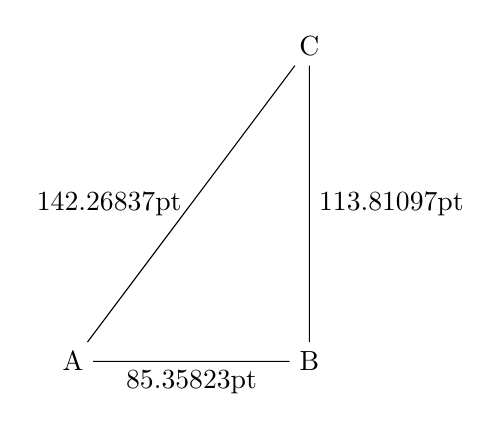
\begin{tikzpicture}
    \node (A) at (0, 0) {A};
    \node (B) at (3, 0) {B};
    \node (C) at (3, 4) {C};
\draw
    let
    \p{AB} = ($ (B) - (A) $),
    \n{AB} = {veclen(\x{AB},\y{AB})},
    \p{AC} = ($ (C) - (A) $),
    \n{AC} = {veclen(\x{AC},\y{AC})},
    \p{BC} = ($ (B) - (C) $),
    \n{BC} = {veclen(\x{BC},\y{BC})}
    in
    (A) -- node[below] {\n{AB}}
    (B) -- node[right] {\n{BC}}
    (C) -- node[left] {\n{AC}} (A);
\end{tikzpicture}
\end{document}
